\section{Model and Methods}
\textbf{---Figure 2 about here---}
\begin{figure}
\centering
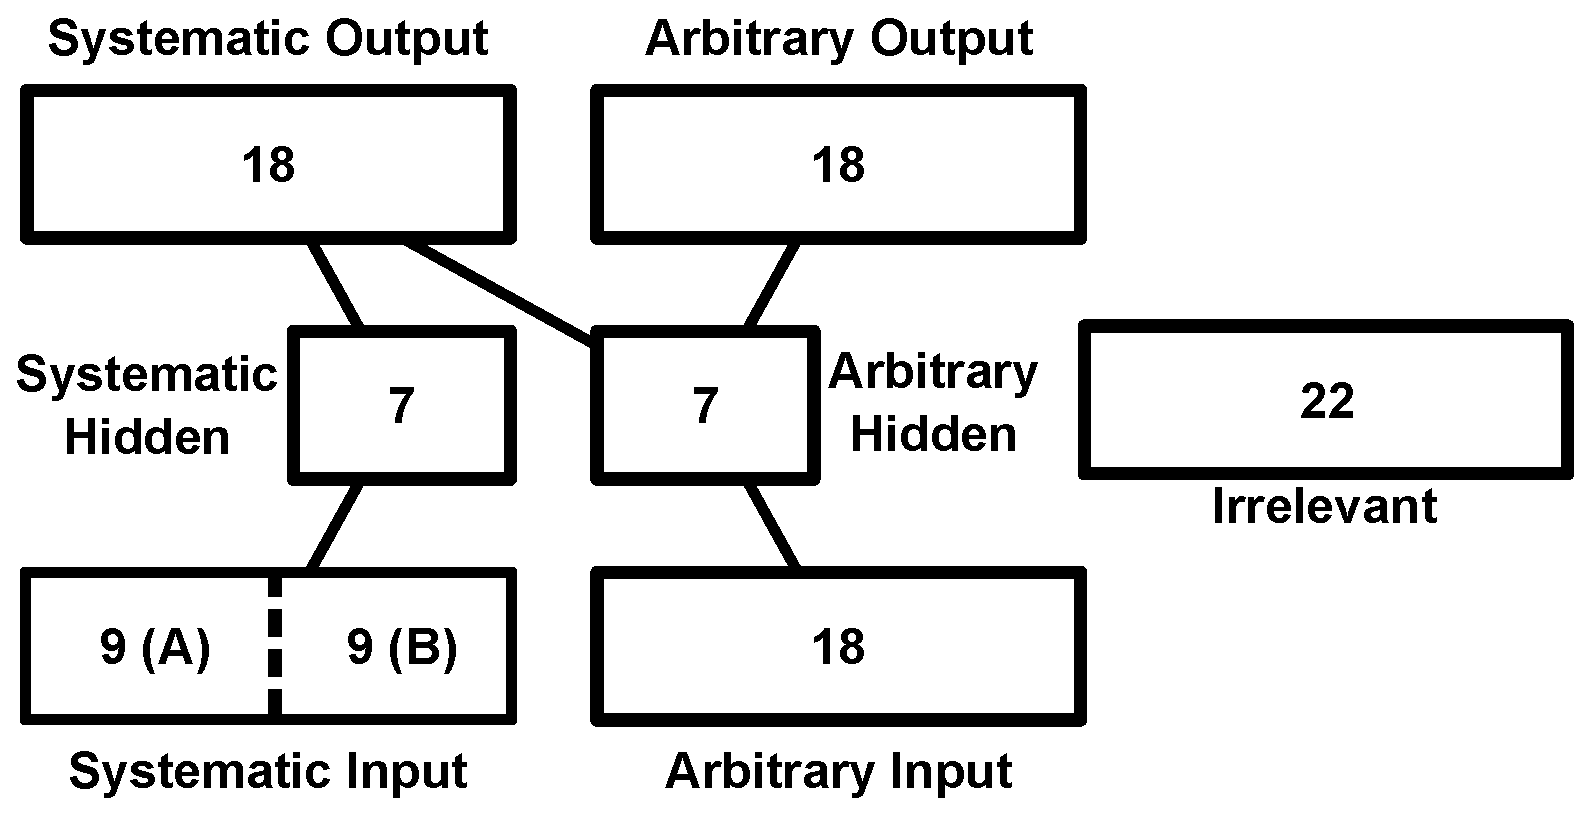
\includegraphics[width=0.75\textwidth]{figures/model_outline.eps}
\caption{\label{fig.model_outline} Schematic outline of the auto-encoder network used to generate the data for the 10 subjects used in subsequent simulations. The model has 36 input units (18 systematic), 14 hidden units (7 systematic), and 36 output units (18 systematic). The 22 irrelevant units are completely disconnected from the network, so receive no input, send no output, and thus learn no representations. They are intended to stand for units that participate in an unrelated network, which are nonetheless anatomically adjacent to our units of interest. See text for full description and motivation.}
\end{figure}


The model we will employ for this analysis is illustrated in Figure 2. It is an auto-encoder network: when presented with an experience in the form of a pattern of activity over its 36 input units, it learns to reproduce that same pattern over its 36 output units. Auto-encoder networks have been used as simple models of human memory, because once they have learned they are capable of both retrieving full information from a partial cue and of generalizing prior learning to new items. In this case, however, we do not intend the model to embody a specific hypothesis about a particular real-world cognitive function. Instead, the model is designed to make explicit the challenges noted in the introduction. 

To this end, the patterns that the model processes are viewed as coming from two different {\em domains}, A and B, corresponding to some cognitive distinction of theoretical import. For instance, A and B might correspond to nouns versus verbs, or animals versus manmade objects, or faces versus non-faces, or any other binary distinction thought to be of potential relevance to behavior.  Each individual item is represented with a unique pattern of activation over input units, and the network's task is simply to generate the same pattern output units. In this sense, there is no explicit representation of the two classes A and B in the inputs, outputs, or network task. The two domains are assumed, however, to be distinguishable from the distribution of input/output properties they possess. Specifically, one subset of input/output units is marginally more likely to be active for items from domain A, while another subset is marginally more likely to be active for items in domain B. We will refer to these subsets together as {\em systematic I/O} (SI/O) units, because they each weakly covary with the representational distinction of interest.  Each item also possesses many {\em arbitrary I/O} (AI/O) units that do not systematically differ between domains.

After the model has learned, it is possible to ``query'' it by presenting an input pattern and generating patterns of activation throughout the rest of the network. As noted earlier, we take the activation at each unit in response to an input as a model analog of the neural response to a stimulus estimated from the BOLD signal at a single voxel in a single individual. Across different training runs, the model will always exhibit the same overt behavior (generating the correct pattern over output units), but arising from different configurations of weights, and hence from different internal representations. Variability in weight configurations and internal representations acquired across different training runs thus provides a model analog of individual variability in the neural representations acquired across the population. To simulate data generated by a functional brain imaging study with, say, 10 participants, we train the model 10 times, and for each trained model, record the pattern of activation generated over all model units by each input pattern (i.e., stimulus). The question we then wish to ask, by applying different statistical methods to the analysis of this synthetic imaging data from a sample of trained models, is the following: where are representations of the domains A and B encoded in the network?

The network architecture is designed so that there are two possible answers to this question. The first answer is that representations of A and B are directly encoded in the activations of systematic I/O units. For all input and output units, the response of a given unit to a particular item is directly specified by the environment, so that these units will always respond to a given stimulus in the same way across training runs. Each systematic I/O unit has a marginally different probability of being active depending upon the domain; in this sense the A units each independently encode a representation of the A domain and the B units encode a representation of the B domain. The relationship between domain and activation is, however, stipulated to be quite loose: for any A item, many A units will be inactive (and vice versa), and so each unit participates in few patterns. Thus different items in the A domain have quite different representations over A units, and the correlation between activation and domain is weak for any individual unit. Nevertheless, each input and output unit responds to stimuli in exactly the same way across model individuals (subject to noise in measurement as explained below). We further stipulate that the A input and output units are anatomical neighbors, as are the B input and output units, and that this anatomical arrangement is exactly the same across individuals. Thus the systematic I/O units individually encode a {\em weak} distinction between A and B that is {\em consistent} across model individuals and is {\em anatomically localized} within input and output layers. 

The second answer is that the representations of A and B domains are encoded in a distributed fashion over a subset of model hidden units. As shown in the Figure, the input units project to the output units by way of two separate hidden layers. The {\em systematic hidden layer} (SH) contains 7 hidden units that receive connections from the systematic input units and send connections to the systematic output units. The {\em arbitrary hidden layer} (AH) also contains 7 units that receive connections from the arbitrary inputs, and send connections to {\em both} the systematic and arbitrary outputs.  The weights are shaped by learning, so each input generates a pattern of activation over both the SH and AH layers, each corresponding to a learned internal representation of the stimulus. The particular way that layers are connected, however, ensures that these internal representations will have specific representational properties. Because the SH layer only passes activation from SI to SO units, it uses it's limited representational capacity to capture the A/B distinction as best it can---items within a domain are represented by quite similar patterns relative items between domains. In contrast, the AH layer receives inputs only from the arbitrary input units and thus uses it's own limited representational capacity to differentiate between each of the items. Consequently, the AH layer acquires distributed internal representations that have very little structure; and the weights in the arbitrary pathways serve to ``memorize'' both the arbitrary features and the idiosyncratic ways that each item differs from its neighbors in systematic properties. In other words, the architecture produces a division of labor in which the SH learns distributed representations that emphasize the A/B distinction, and the AH does not. A good method, then, should identify SH units as important for representing the domains.

In addition, there are 22 completely irrelevant units. These units are positioned anatomically adjacent to the SH and AH units but are completely unrelated to the behavior of the network. Because they receive no input, they never activate. They are nevertheless important to the simulations that follow: they stand for units that participate in some other network altogether, yet are anatomic neighbors to the SH and AH units. Acknowledging challenges 3 and 4, these units are also measured, and might even be interspersed with the representations we care to discover.

\textbf{---Figure 3 about here---}
\begin{figure}
\centering
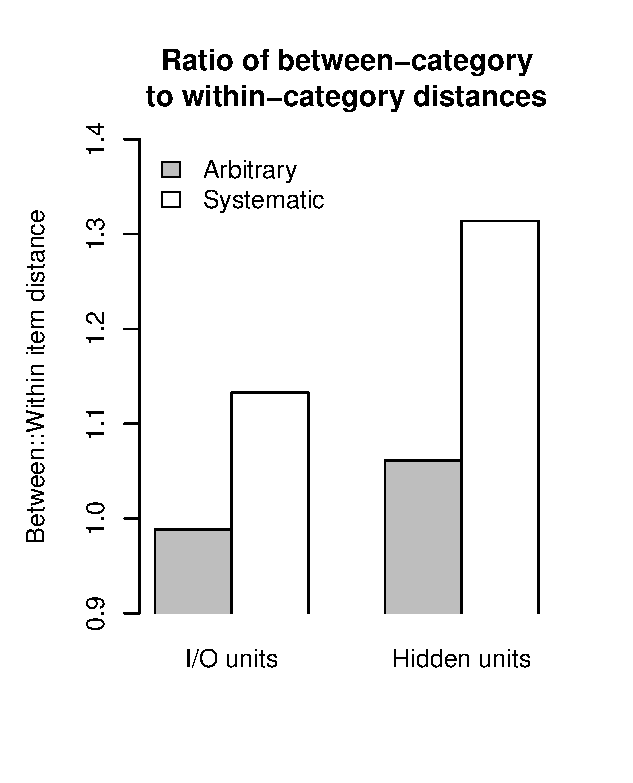
\includegraphics[width=0.5\textwidth]{figures/between_within_dist.eps}
\caption{\label{fig.between_within_dist} The dissimilarity of two distributed representations can be quantified as a distance. Distributed representations that have large distances between items from domains A and B in our model, relative to the distances between items of the same domain, will contain information relevant to training a classifier to determine which domain an example belongs to. Here, we plotted the ratio of between::within group distances for the representations over different sets of units in our network, averaged over the 10 subjects used in subsequent analyses. }
\end{figure}

With this general understanding of the model behavior, let's consider how it makes explicit the four challenges for brain imaging noted earlier. First, although the same representational structure is observed across all network runs, the particular way it is expressed across individual units is essentially arbitrary for the reasons noted in the introduction (challenge 1). Second, the mean activations of SH units taken independently do not systematically differ for items in the A and B domains: to find the important structure, one must consider the pattern evoked over multiple units (challenge 2). Third, the functional architecture of the model shown in Figure 2 can be anatomically arranged in many different ways (challenge 3). To make this issue explicit, we consider two different topographic arrangements of the functional model. In the first, units within the same layer are always situated as anatomical neighbors, so that the representations encoded by the SH and the AH layers are {\em anatomically localized}. In the second arrangement, we assume that the SH units are {\em dispersed} amongst the AH units, differently in each model individual. In the results we will consider how well each method identifies the SH units as a function of whether they are localized or dispersed. Finally, the model captures the idea that the units of interest constitute only a small proportion of all the units measured (challenge 4). In the model itself, most of the units are dedicated to processing arbitrary patterns (18 arbitrary I/O units and 7 arbitrary hidden units). The next largest set of units that participate in the network are the systematic I/O units that weakly but consistently encode the category structure. The units of greatest interest, the SH units, constitute just 6\% of the measured units. 

\subsection{Summary} 

Though very simple, this auto-encoder network captures each of the challenges noted in the introduction: it acquires distributed internal representations that express representational structure of interest; the way the structure is coded across units varies in different individual models; the structure cannot be discerned from the activations of single units but arises in patterns over multiple units; the relationship between the functional architecture and the underlying model topography can be opaque; and the units that encode the structure we wish to discover are buried in a large number of other measurements. The question we now address is how well different analysis methods fare at discovering representational structure across both systematic I/O units and the SH units, when they are applied to data generated from a sample of model training runs.
